Pour la sélection des composants, en plus des éléments imposés par le projet, nous avons décidé de concevoir un modèle 3D, d'opter pour l'utilisation d'une manette SONY PS5 et d'employer des câbles femelle-femelle.

\subsection{Choix de la manette}
Le choix de la manette s'est imposé en raison de sa précision supérieure par rapport à la télécommande. En effet, les deux gâchettes arrière émettent des valeurs comprises entre 0 et 255, tandis que les joysticks génèrent des valeurs entre 0 et 180. Couplées aux signaux PWM, ces caractéristiques nous ont offert une précision accrue tant au niveau de la vitesse que des manœuvres.

Quant au code de la manette, nous avons initialement utilisé la bibliothèque de bas niveau libevdev, spécifique à la manette PS5. Toutefois, nous avons ultérieurement opté pour la bibliothèque SDL 2.0, plus haut niveau, rendant ainsi notre code compatible avec toutes les manettes.

\subsection{Modèle 3D}
En ce qui concerne le choix du modèle 3D, il s'est principalement orienté vers des considérations esthétiques. Nous avons privilégié un modèle compact qui évoquerait une véritable voiture télécommandée.

\begin{figure}[h]
    \centering
    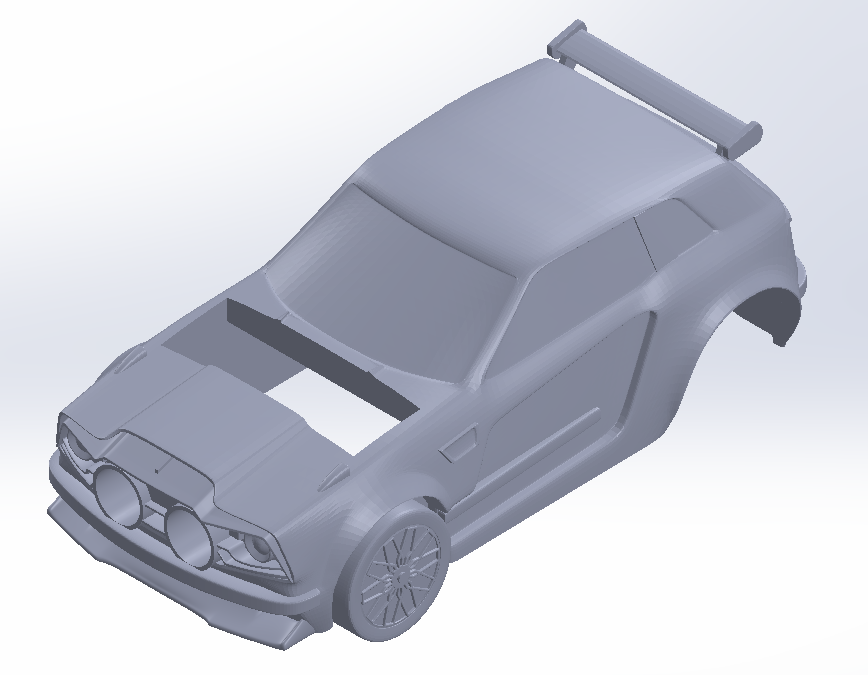
\includegraphics[width=0.3\textwidth]{images/solidworks/solidworks1.png}
    \caption{Vue principale conception 3D}
    \label{fig:Vue principale conception 3D}
\end{figure}

\begin{figure}[h]
    \centering
    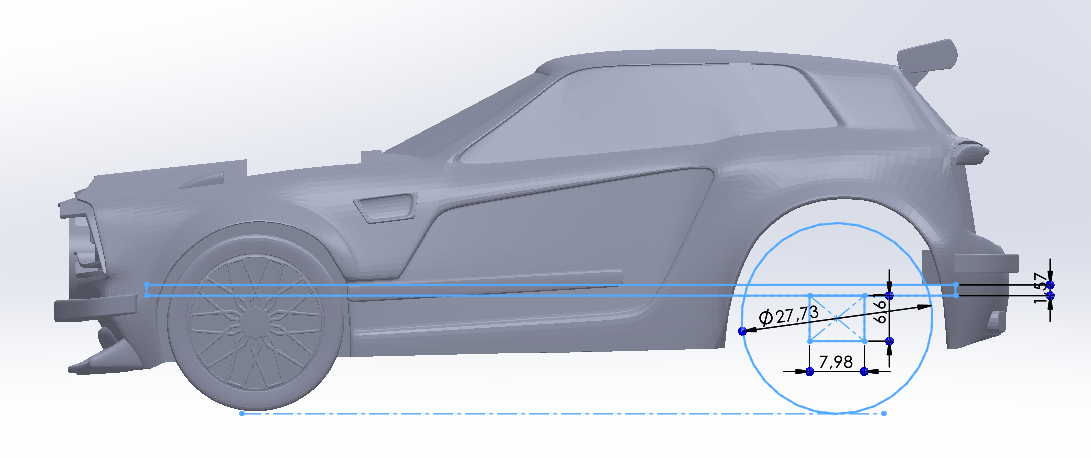
\includegraphics[width=0.3\textwidth]{images/solidworks/solidworks3.png}
    \caption{Vue de côté conception 3D}
    \label{fig:Vue de côté conception 3D}
\end{figure}

\begin{figure}[h]
    \centering
    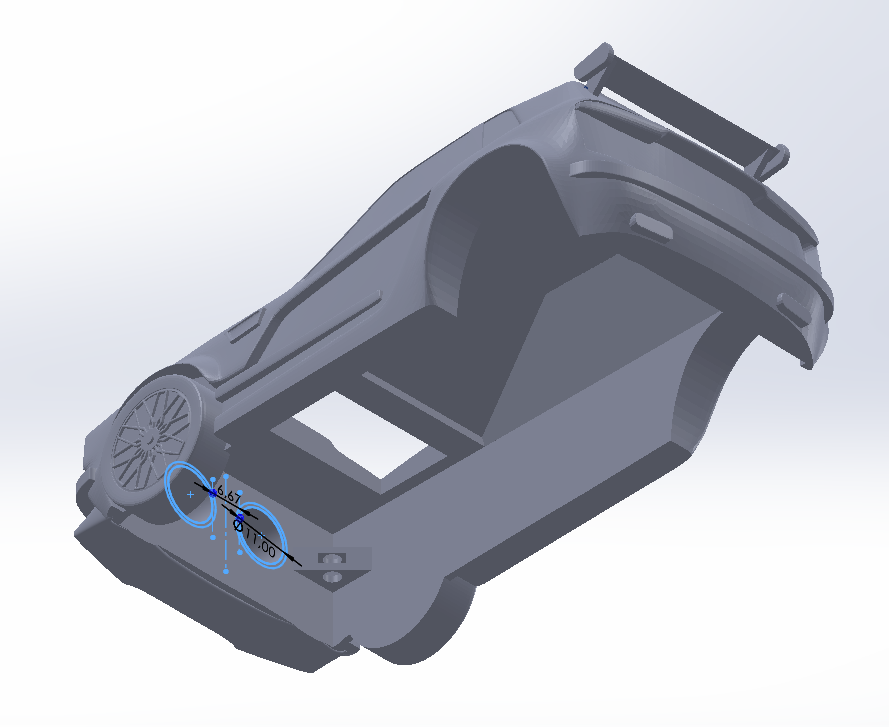
\includegraphics[width=0.3\textwidth]{images/solidworks/solidworks4.png}
    \caption{Vue du dessous conception 3D}
    \label{fig:Vue du dessous conception 3D}
\end{figure}

\newpage